% Written by paper/figures/src/v6_more.py; edit the script, not this file.
\begin{figure}[p]
  \centering
  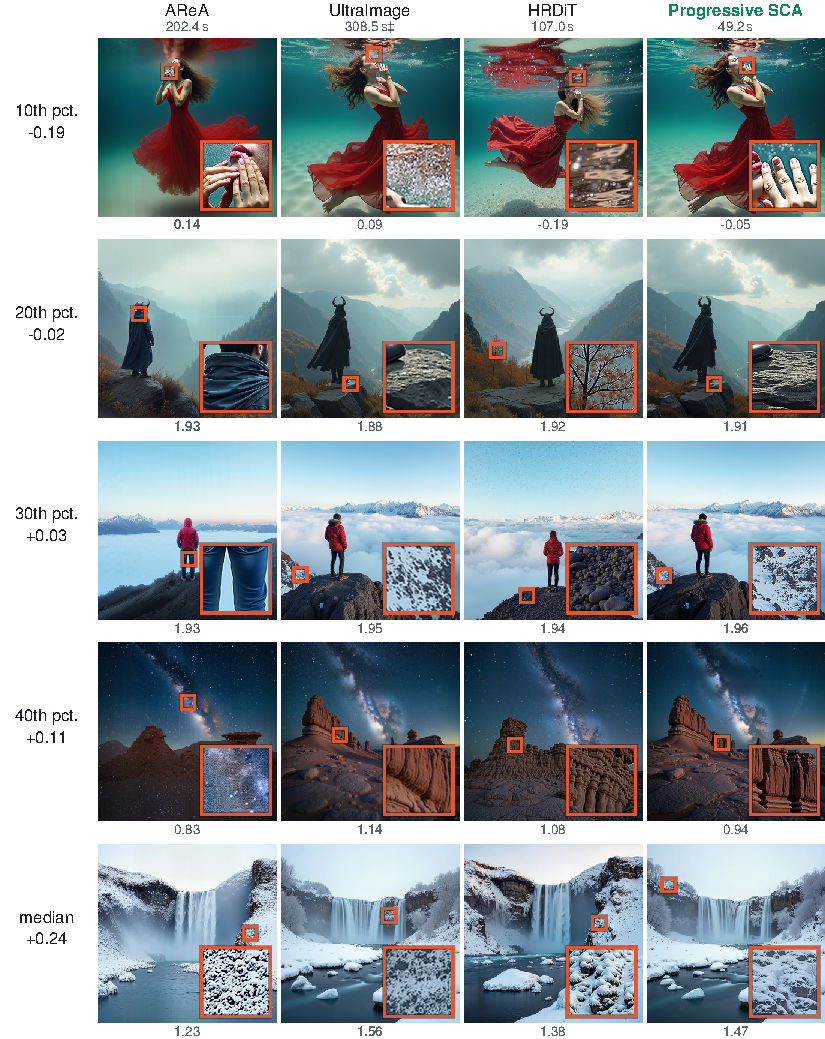
\includegraphics{figures/v6/deciles_a.pdf}
  \caption{\textbf{Whole-image comparison at every decile of progressive \sca{}'s ImageReward gain over AReA (10th to 50th percentile).} Rows: the evaluation prompts at the 10th, 20th, \ldots, 90th percentile (nearest rank) of the paired ImageReward difference, progressive \sca{} minus AReA, over the 195 prompts at seed~0; the label gives the difference. Under each image its ImageReward (best bold); insets show each image's highest-detail $256^2$ window at 1:1; times are clean seconds per $4096^2$ image (\textdaggerdbl{} campaign mean). Figure~\ref{fig:deciles_b} continues.}
  \label{fig:deciles_a}
\end{figure}
\begin{figure}[p]
  \centering
  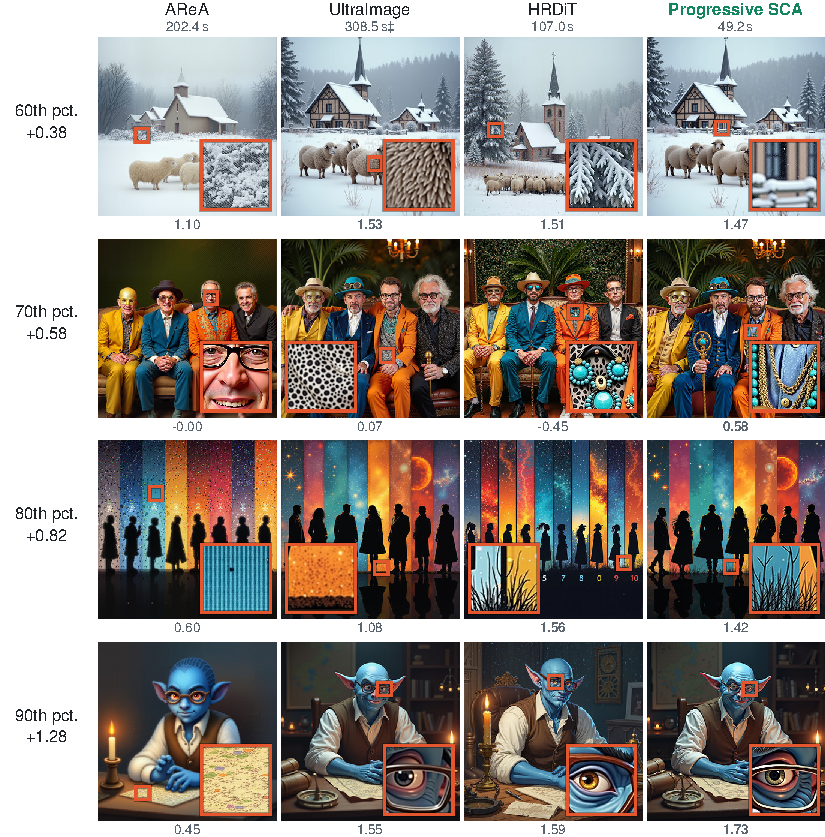
\includegraphics{figures/v6/deciles_b.pdf}
  \caption{\textbf{Whole-image comparison at every decile of progressive \sca{}'s ImageReward gain over AReA (60th to 90th percentile).} Rows: the evaluation prompts at the 10th, 20th, \ldots, 90th percentile (nearest rank) of the paired ImageReward difference, progressive \sca{} minus AReA, over the 195 prompts at seed~0; the label gives the difference. Under each image its ImageReward (best bold); insets show each image's highest-detail $256^2$ window at 1:1; times are clean seconds per $4096^2$ image (\textdaggerdbl{} campaign mean).}
  \label{fig:deciles_b}
\end{figure}
